
\documentclass[10pt,twocolumn,letterpaper]{article}
% ICCV Rules:
% 8 page limit (6 free + 2 paid)
% 10MB pdf file size limit
% 30MB supplementary materials file size limit (PDF or ZIP)

\usepackage{iccv}
\usepackage[pagebackref=true,breaklinks=true,letterpaper=true,colorlinks,bookmarks=false]{hyperref}
\usepackage{times}
\usepackage{epsfig}
\usepackage{graphicx}
\usepackage{amsmath}
\usepackage{amssymb}
\usepackage{amsfonts}
\usepackage{algorithm}
\usepackage{algorithmic}

% Needed for getting formulas in dia diagrams.
\usepackage{pstricks}
\usepackage{tikz}

\usepackage{mydefs}

% \cvprfinalcopy % *** Uncomment this line for the final submission

\def\iccvPaperID{257} % *** Enter the CVPR Paper ID here
\def\httilde{\mbox{\tt\raisebox{-.5ex}{\symbol{126}}}}

% Pages are numbered in submission mode, and unnumbered in camera-ready
\ificcvfinal\pagestyle{empty}\fi
\begin{document}

%\title{Accelerating $\ell_1$-Minimization Using Many-Core CPUs/GPUs \\ and Application to Face Recognition
%\title{Efficient Parallelization of Sparse Representation for Face Recognition}
%\thanks{Corresponding author: . This work was partially supported by ARO MURI W911NF-06-1-0076.}}
%\title{Many-Core Parallelization of $\ell_1$-Minimization for Face Recognition
\title{Parallelization of Fast $\ell_1$-Minimization for Face Recognition
%\thanks{Corresponding author: . This work was partially supported by ARO MURI W911NF-06-1-0076.}
}

\author{First Author\\
Institution1\\
Institution1 address\\
{\tt\small firstauthor@i1.org}
% For a paper whose authors are all at the same institution,
% omit the following lines up until the closing ``}''.
% Additional authors and addresses can be added with ``\and'',
% just like the second author.
% To save space, use either the email address or home page, not both
\and
Second Author\\
Institution2\\
First line of institution2 address\\
{\small\url{http://www.author.org/~second}}
}

\maketitle

\begin{abstract}

\end{abstract}

\section{Introduction} 
$\ell_1$-minimization ($\ell_1$-min) has received much attention in recent
years due to important applications in compressive sensing
\cite{BrucksteinA2007} and sparse representation \cite{WrightJ2010-PIEEE}.  
$\ell_1$-min refers to finding the minimum $\ell$-norm solution to an
underdetermined linear system $\bb=A\xx$:
\begin{equation}
\min \|\xx\|_1\quad \mbox{ subj. to }\quad \bb = A\xx.
\label{eq:l1min}
\end{equation}
It is now well established that, under certain conditions
\cite{CandesE2005-IT_1,DonohoD2004}, the minimum $\ell_1$-norm solution is also
the \emph{sparsest} solution to the system \eqref{eq:l1min}.

Among its many applications, $\ell_1$-min has been recently used to reformulate
image-based face recognition as a sparse representation problem
\cite{WrightJ2009-PAMI}.  If we stack the training images of $K$ subject
classes $(A_1\in\Re^{d\times n_1}, \cdots, A_K\in\Re^{d\times n_K})$ into the
columns of a matrix $A = [A_1, \cdots, A_K]\in\Re^{d\times n}$, given a new
query image in the same vector form $\bb\in\Re^d$, \emph{sparsity-based
classification} (SBC) solves the following minimization problem:
\begin{equation}
\min_{\xx, \ee} \| \xx \|_1 + \|\ee\|_1 \quad \subj \quad \bb = A \xx + \ee.
\label{eq:l1min_denoise}
\end{equation}
If the sparsest solutions for $\x$ and $\e$ are recovered, $\ee$ provides a
means to compensate for pixels that are corrupted due to occlusion of some part of the query
image, and the dominant nonzero coefficients of $\xx$ reveal the membership of
$\bb$ based on the training image labels associated with $A$.  Since $A$ ideally
contains many images per user taken under different illuminations, 
$A\x$ also acts as a linear illumination model for the test image $\bb$.

In this paper, we study parallelization of $\ell$-min on many-core CPU and GPU
architectures. Although $\ell_1$-min \eqref{eq:l1min} is a convex
program, conventional algorithms such as interior-point methods
\cite{ChenS2001-SIAM,TibshiraniR1996} are known to suffer from poor scalability
for large-scale applications such as face recognition. Recently, a number of
accelerated algorithms have been proposed that explicitly take advantage of
the special structure of $\ell_1$-min problems
\cite{LorisI2009,YangA2010-ICIP}. We investigate parallelization of a
state-of-the-art $\ell_1$-min solution based on the classical framework of
\emph{augmented Lagrange multiplier} (ALM) \cite{BertsekasD2003,YangA2010-ICIP}.

While solving \eqref{eq:l1min_denoise} can achieve exceptional
recognition accuracy on public databases, its success relies on the assumption
that the query image is well aligned with the training images. In
\cite{WagnerA2009-CVPR}, the framework of SBC was extended to iteratively align
a query image to one subject class. The face alignment algorithm in turn solves
the following minimization problem:
\begin{equation}
\hat{\tau}_i = \arg\min_{\xx, \ee, \tau_i} \|\ee\|_1\quad \mbox{subj. to}\quad \tilde\bb\circ\tau_i = A_i\xx + \ee,
\label{eq:l1min_alignment}
\end{equation}
where $\tau_i\in T$ is in a finite-dimensional group $T$ of transformations
(e.g., affine or homography) acting on the image domain, which aligns $\tilde\bb$
with the training images from the $i$-th class $A_i$. The algorithm 
extends Lucas-Kanade iterative alignment \cite{LucasB1981} to both to use the
$\ell_1$ norm as a robust error function, and also simultaneously 
to estimate the illumination model $A\x$.  
The original solution \cite{WagnerA2009-CVPR} was implemented based 
on standard interior-point
methods, and its speed has been since improved by ALM in a more recent paper
\cite{WagnerA2011-PAMI}. However, primarily due the high per-user cost
of the alignment step, the recognition system was still not fast enough
for real-time recognition against datasets of hundreds of users.
In this paper, in addition to solving the generic
$\ell_1$-min objectives \eqref{eq:l1min} and \eqref{eq:l1min_denoise}, we 
discuss how to properly accelerate the iterative face alignment step
\eqref{eq:l1min_alignment} on multi-core CPUs and GPUs. 

Finally, we present extensive benchmark to compare the performance of the
generic ALM $\ell_1$-min algorithm and the corresponding face recognition
routines on massively parallel CPUs and GPUs.  To this end, the face
recognition system has been fully implemented on a state-of-the-art
workstation, as shown in Figure \ref{fig:pipeline}. 
Since the parallelization of any algorithm
is highly dependent on the target hardware, we will give a brief overview of
the architecture of our test system in detail in Section
\ref{sec:parallelism}.  We will show that a highly accurate and robust face
recognition system can be constructed to recognize face images from a 
database of several hundred subjects quickly enough to be practical for
access control applications. 
Note that for applications targeting thousands of users or more, it would likely be
necessary to distribute the work over a network of machines; this paper
focuses on the (shared memory) parallelism available in a single machine.
The C++ source code of our implementations, which target Nvidia's CUDA GPU architecture
will be made available for evaluation by other researchers.
\begin{figure}
\centering
{\tiny % Graphic for TeX using PGF
% Title: pipeline_simplified.dia
% Creator: Dia v0.97-pre3
% CreationDate: Mon Feb 14 03:20:49 2011
% For: awagner
% \usepackage{tikz}
% The following commands are not supported in PSTricks at present
% We define them conditionally, so when they are implemented,
% this pgf file will use them.
\ifx\du\undefined
  \newlength{\du}
\fi
\setlength{\du}{15\unitlength}
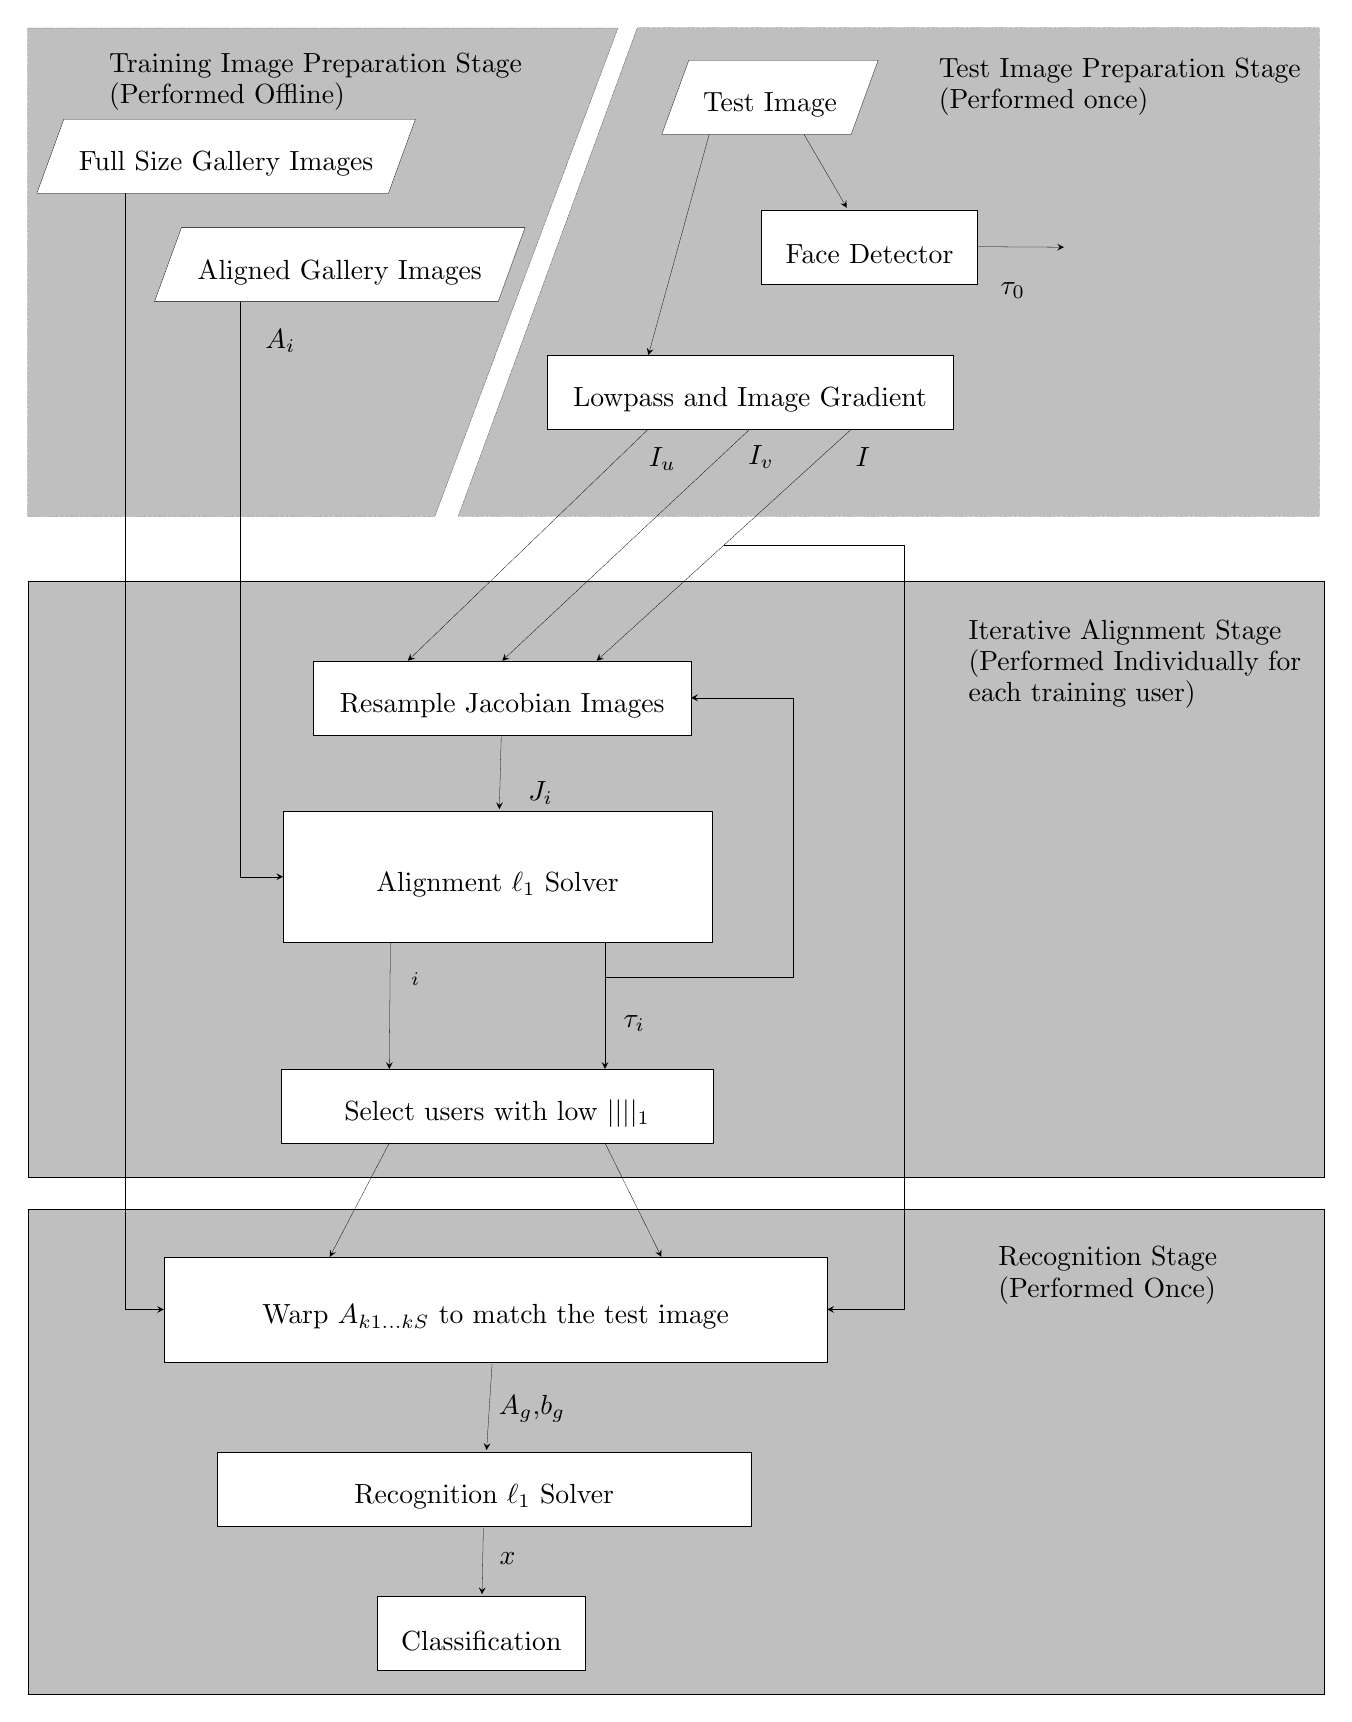
\begin{tikzpicture}
\pgftransformxscale{0.494667}
\pgftransformyscale{-0.494667}
\definecolor{dialinecolor}{rgb}{0.000000, 0.000000, 0.000000}
\pgfsetstrokecolor{dialinecolor}
\definecolor{dialinecolor}{rgb}{1.000000, 1.000000, 1.000000}
\pgfsetfillcolor{dialinecolor}
% setfont left to latex
\definecolor{dialinecolor}{rgb}{0.000000, 0.000000, 0.000000}
\pgfsetstrokecolor{dialinecolor}
\node[anchor=west] at (24.925000\du,42.952500\du){};
% setfont left to latex
\definecolor{dialinecolor}{rgb}{0.000000, 0.000000, 0.000000}
\pgfsetstrokecolor{dialinecolor}
\node[anchor=west] at (24.925000\du,42.952500\du){};
% setfont left to latex
\definecolor{dialinecolor}{rgb}{0.000000, 0.000000, 0.000000}
\pgfsetstrokecolor{dialinecolor}
\node[anchor=west] at (24.925000\du,42.952500\du){};
\definecolor{dialinecolor}{rgb}{0.749020, 0.749020, 0.749020}
\pgfsetfillcolor{dialinecolor}
\fill (6.494040\du,27.943300\du)--(6.494040\du,43.255071\du)--(39.770015\du,43.255071\du)--(39.770015\du,27.943300\du)--cycle;
\pgfsetlinewidth{0.100000\du}
\pgfsetdash{{\pgflinewidth}{0.200000\du}}{0cm}
\pgfsetdash{{\pgflinewidth}{0.200000\du}}{0cm}
\pgfsetmiterjoin
\definecolor{dialinecolor}{rgb}{0.000000, 0.000000, 0.000000}
\pgfsetstrokecolor{dialinecolor}
\draw (6.494040\du,27.943300\du)--(6.494040\du,43.255071\du)--(39.770015\du,43.255071\du)--(39.770015\du,27.943300\du)--cycle;
% setfont left to latex
\definecolor{dialinecolor}{rgb}{0.000000, 0.000000, 0.000000}
\pgfsetstrokecolor{dialinecolor}
\node at (23.132027\du,35.794186\du){};
\definecolor{dialinecolor}{rgb}{0.749020, 0.749020, 0.749020}
\pgfsetfillcolor{dialinecolor}
\fill (6.494040\du,44.061200\du)--(6.494040\du,56.519596\du)--(39.770015\du,56.519596\du)--(39.770015\du,44.061200\du)--cycle;
\pgfsetlinewidth{0.100000\du}
\pgfsetdash{{\pgflinewidth}{0.200000\du}}{0cm}
\pgfsetdash{{\pgflinewidth}{0.200000\du}}{0cm}
\pgfsetmiterjoin
\definecolor{dialinecolor}{rgb}{0.000000, 0.000000, 0.000000}
\pgfsetstrokecolor{dialinecolor}
\draw (6.494040\du,44.061200\du)--(6.494040\du,56.519596\du)--(39.770015\du,56.519596\du)--(39.770015\du,44.061200\du)--cycle;
% setfont left to latex
\definecolor{dialinecolor}{rgb}{0.000000, 0.000000, 0.000000}
\pgfsetstrokecolor{dialinecolor}
\node at (23.132027\du,50.485398\du){};
% setfont left to latex
\definecolor{dialinecolor}{rgb}{0.000000, 0.000000, 0.000000}
\pgfsetstrokecolor{dialinecolor}
\node[anchor=west] at (23.132000\du,35.599200\du){};
% setfont left to latex
\definecolor{dialinecolor}{rgb}{0.000000, 0.000000, 0.000000}
\pgfsetstrokecolor{dialinecolor}
\node[anchor=west] at (23.132000\du,35.599200\du){};
% setfont left to latex
\definecolor{dialinecolor}{rgb}{0.000000, 0.000000, 0.000000}
\pgfsetstrokecolor{dialinecolor}
\node[anchor=west] at (30.406100\du,29.259100\du){Iterative Alignment Stage};
% setfont left to latex
\definecolor{dialinecolor}{rgb}{0.000000, 0.000000, 0.000000}
\pgfsetstrokecolor{dialinecolor}
\node[anchor=west] at (30.406100\du,30.059100\du){(Performed Individually for};
% setfont left to latex
\definecolor{dialinecolor}{rgb}{0.000000, 0.000000, 0.000000}
\pgfsetstrokecolor{dialinecolor}
\node[anchor=west] at (30.406100\du,30.859100\du){each training user)};
% setfont left to latex
\definecolor{dialinecolor}{rgb}{0.000000, 0.000000, 0.000000}
\pgfsetstrokecolor{dialinecolor}
\node[anchor=west] at (31.173700\du,45.350700\du){Recognition Stage};
% setfont left to latex
\definecolor{dialinecolor}{rgb}{0.000000, 0.000000, 0.000000}
\pgfsetstrokecolor{dialinecolor}
\node[anchor=west] at (31.173700\du,46.150700\du){(Performed Once)};
\pgfsetlinewidth{0.100000\du}
\pgfsetdash{{\pgflinewidth}{0.200000\du}}{0cm}
\pgfsetdash{{\pgflinewidth}{0.200000\du}}{0cm}
\pgfsetmiterjoin
\pgfsetbuttcap
\definecolor{dialinecolor}{rgb}{0.749020, 0.749020, 0.749020}
\pgfsetfillcolor{dialinecolor}
\fill (6.494040\du,13.746400\du)--(21.645100\du,13.746400\du)--(16.943000\du,26.285100\du)--(6.494040\du,26.285100\du)--cycle;
\definecolor{dialinecolor}{rgb}{0.000000, 0.000000, 0.000000}
\pgfsetstrokecolor{dialinecolor}
\draw (6.494040\du,13.746400\du)--(21.645100\du,13.746400\du)--(16.943000\du,26.285100\du)--(6.494040\du,26.285100\du)--cycle;
% setfont left to latex
\definecolor{dialinecolor}{rgb}{0.000000, 0.000000, 0.000000}
\pgfsetstrokecolor{dialinecolor}
\node[anchor=west] at (8.342710\du,14.710900\du){Training Image Preparation Stage};
% setfont left to latex
\definecolor{dialinecolor}{rgb}{0.000000, 0.000000, 0.000000}
\pgfsetstrokecolor{dialinecolor}
\node[anchor=west] at (8.342710\du,15.510900\du){(Performed Offline)};
\pgfsetlinewidth{0.100000\du}
\pgfsetdash{{\pgflinewidth}{0.200000\du}}{0cm}
\pgfsetdash{{\pgflinewidth}{0.200000\du}}{0cm}
\pgfsetmiterjoin
\pgfsetbuttcap
\definecolor{dialinecolor}{rgb}{0.749020, 0.749020, 0.749020}
\pgfsetfillcolor{dialinecolor}
\fill (22.141100\du,13.740100\du)--(39.649500\du,13.740100\du)--(39.649500\du,26.278900\du)--(17.545800\du,26.278900\du)--cycle;
\definecolor{dialinecolor}{rgb}{0.000000, 0.000000, 0.000000}
\pgfsetstrokecolor{dialinecolor}
\draw (22.141100\du,13.740100\du)--(39.649500\du,13.740100\du)--(39.649500\du,26.278900\du)--(17.545800\du,26.278900\du)--cycle;
% setfont left to latex
\definecolor{dialinecolor}{rgb}{0.000000, 0.000000, 0.000000}
\pgfsetstrokecolor{dialinecolor}
\node[anchor=west] at (29.642500\du,14.831400\du){Test Image Preparation Stage};
% setfont left to latex
\definecolor{dialinecolor}{rgb}{0.000000, 0.000000, 0.000000}
\pgfsetstrokecolor{dialinecolor}
\node[anchor=west] at (29.642500\du,15.631400\du){(Performed once)};
\definecolor{dialinecolor}{rgb}{1.000000, 1.000000, 1.000000}
\pgfsetfillcolor{dialinecolor}
\fill (23.464443\du,14.572100\du)--(28.325620\du,14.572100\du)--(27.634076\du,16.472100\du)--(22.772900\du,16.472100\du)--cycle;
\pgfsetlinewidth{0.100000\du}
\pgfsetdash{}{0pt}
\pgfsetdash{}{0pt}
\pgfsetmiterjoin
\definecolor{dialinecolor}{rgb}{0.000000, 0.000000, 0.000000}
\pgfsetstrokecolor{dialinecolor}
\draw (23.464443\du,14.572100\du)--(28.325620\du,14.572100\du)--(27.634076\du,16.472100\du)--(22.772900\du,16.472100\du)--cycle;
% setfont left to latex
\definecolor{dialinecolor}{rgb}{0.000000, 0.000000, 0.000000}
\pgfsetstrokecolor{dialinecolor}
\node at (25.549260\du,15.717100\du){Test Image};
\definecolor{dialinecolor}{rgb}{1.000000, 1.000000, 1.000000}
\pgfsetfillcolor{dialinecolor}
\fill (13.826900\du,29.990700\du)--(13.826900\du,31.890700\du)--(23.521900\du,31.890700\du)--(23.521900\du,29.990700\du)--cycle;
\pgfsetlinewidth{0.100000\du}
\pgfsetdash{}{0pt}
\pgfsetdash{}{0pt}
\pgfsetmiterjoin
\definecolor{dialinecolor}{rgb}{0.000000, 0.000000, 0.000000}
\pgfsetstrokecolor{dialinecolor}
\draw (13.826900\du,29.990700\du)--(13.826900\du,31.890700\du)--(23.521900\du,31.890700\du)--(23.521900\du,29.990700\du)--cycle;
% setfont left to latex
\definecolor{dialinecolor}{rgb}{0.000000, 0.000000, 0.000000}
\pgfsetstrokecolor{dialinecolor}
\node at (18.674400\du,31.135700\du){Resample Jacobian Images};
\definecolor{dialinecolor}{rgb}{1.000000, 1.000000, 1.000000}
\pgfsetfillcolor{dialinecolor}
\fill (13.050000\du,33.850000\du)--(13.050000\du,37.221200\du)--(24.058800\du,37.221200\du)--(24.058800\du,33.850000\du)--cycle;
\pgfsetlinewidth{0.100000\du}
\pgfsetdash{}{0pt}
\pgfsetdash{}{0pt}
\pgfsetmiterjoin
\definecolor{dialinecolor}{rgb}{0.000000, 0.000000, 0.000000}
\pgfsetstrokecolor{dialinecolor}
\draw (13.050000\du,33.850000\du)--(13.050000\du,37.221200\du)--(24.058800\du,37.221200\du)--(24.058800\du,33.850000\du)--cycle;
% setfont left to latex
\definecolor{dialinecolor}{rgb}{0.000000, 0.000000, 0.000000}
\pgfsetstrokecolor{dialinecolor}
\node at (18.554400\du,35.730600\du){Alignment $\ell_1$ Solver};
\pgfsetlinewidth{0.100000\du}
\pgfsetdash{}{0pt}
\pgfsetdash{}{0pt}
\pgfsetbuttcap
{
\definecolor{dialinecolor}{rgb}{0.000000, 0.000000, 0.000000}
\pgfsetfillcolor{dialinecolor}
% was here!!!
\pgfsetarrowsend{stealth}
\definecolor{dialinecolor}{rgb}{0.000000, 0.000000, 0.000000}
\pgfsetstrokecolor{dialinecolor}
\draw (18.648326\du,31.939104\du)--(18.599693\du,33.801294\du);
}
% setfont left to latex
\definecolor{dialinecolor}{rgb}{0.000000, 0.000000, 0.000000}
\pgfsetstrokecolor{dialinecolor}
\node[anchor=west] at (11.250000\du,34.890000\du){};
\definecolor{dialinecolor}{rgb}{1.000000, 1.000000, 1.000000}
\pgfsetfillcolor{dialinecolor}
\fill (19.817600\du,22.143000\du)--(19.817600\du,24.043000\du)--(30.250100\du,24.043000\du)--(30.250100\du,22.143000\du)--cycle;
\pgfsetlinewidth{0.100000\du}
\pgfsetdash{}{0pt}
\pgfsetdash{}{0pt}
\pgfsetmiterjoin
\definecolor{dialinecolor}{rgb}{0.000000, 0.000000, 0.000000}
\pgfsetstrokecolor{dialinecolor}
\draw (19.817600\du,22.143000\du)--(19.817600\du,24.043000\du)--(30.250100\du,24.043000\du)--(30.250100\du,22.143000\du)--cycle;
% setfont left to latex
\definecolor{dialinecolor}{rgb}{0.000000, 0.000000, 0.000000}
\pgfsetstrokecolor{dialinecolor}
\node at (25.033850\du,23.288000\du){Lowpass and Image Gradient};
\definecolor{dialinecolor}{rgb}{1.000000, 1.000000, 1.000000}
\pgfsetfillcolor{dialinecolor}
\fill (25.332900\du,18.409900\du)--(25.332900\du,20.309900\du)--(30.875400\du,20.309900\du)--(30.875400\du,18.409900\du)--cycle;
\pgfsetlinewidth{0.100000\du}
\pgfsetdash{}{0pt}
\pgfsetdash{}{0pt}
\pgfsetmiterjoin
\definecolor{dialinecolor}{rgb}{0.000000, 0.000000, 0.000000}
\pgfsetstrokecolor{dialinecolor}
\draw (25.332900\du,18.409900\du)--(25.332900\du,20.309900\du)--(30.875400\du,20.309900\du)--(30.875400\du,18.409900\du)--cycle;
% setfont left to latex
\definecolor{dialinecolor}{rgb}{0.000000, 0.000000, 0.000000}
\pgfsetstrokecolor{dialinecolor}
\node at (28.104150\du,19.554900\du){Face Detector};
\definecolor{dialinecolor}{rgb}{1.000000, 1.000000, 1.000000}
\pgfsetfillcolor{dialinecolor}
\fill (9.987950\du,45.295200\du)--(9.987950\du,47.995200\du)--(27.017950\du,47.995200\du)--(27.017950\du,45.295200\du)--cycle;
\pgfsetlinewidth{0.100000\du}
\pgfsetdash{}{0pt}
\pgfsetdash{}{0pt}
\pgfsetmiterjoin
\definecolor{dialinecolor}{rgb}{0.000000, 0.000000, 0.000000}
\pgfsetstrokecolor{dialinecolor}
\draw (9.987950\du,45.295200\du)--(9.987950\du,47.995200\du)--(27.017950\du,47.995200\du)--(27.017950\du,45.295200\du)--cycle;
% setfont left to latex
\definecolor{dialinecolor}{rgb}{0.000000, 0.000000, 0.000000}
\pgfsetstrokecolor{dialinecolor}
\node at (18.502950\du,46.840200\du){Warp $A_{k1 \ldots kS}$ to match the test image};
\definecolor{dialinecolor}{rgb}{1.000000, 1.000000, 1.000000}
\pgfsetfillcolor{dialinecolor}
\fill (15.470400\du,54.006500\du)--(15.470400\du,55.906500\du)--(20.802900\du,55.906500\du)--(20.802900\du,54.006500\du)--cycle;
\pgfsetlinewidth{0.100000\du}
\pgfsetdash{}{0pt}
\pgfsetdash{}{0pt}
\pgfsetmiterjoin
\definecolor{dialinecolor}{rgb}{0.000000, 0.000000, 0.000000}
\pgfsetstrokecolor{dialinecolor}
\draw (15.470400\du,54.006500\du)--(15.470400\du,55.906500\du)--(20.802900\du,55.906500\du)--(20.802900\du,54.006500\du)--cycle;
% setfont left to latex
\definecolor{dialinecolor}{rgb}{0.000000, 0.000000, 0.000000}
\pgfsetstrokecolor{dialinecolor}
\node at (18.136650\du,55.151500\du){Classification};
% setfont left to latex
\definecolor{dialinecolor}{rgb}{0.000000, 0.000000, 0.000000}
\pgfsetstrokecolor{dialinecolor}
\node[anchor=west] at (28.104200\du,19.359900\du){};
\pgfsetlinewidth{0.100000\du}
\pgfsetdash{}{0pt}
\pgfsetdash{}{0pt}
\pgfsetbuttcap
{
\definecolor{dialinecolor}{rgb}{0.000000, 0.000000, 0.000000}
\pgfsetfillcolor{dialinecolor}
% was here!!!
\pgfsetarrowsend{stealth}
\definecolor{dialinecolor}{rgb}{0.000000, 0.000000, 0.000000}
\pgfsetstrokecolor{dialinecolor}
\draw (25.033800\du,24.043000\du)--(18.674400\du,29.990700\du);
}
\pgfsetlinewidth{0.100000\du}
\pgfsetdash{}{0pt}
\pgfsetdash{}{0pt}
\pgfsetbuttcap
{
\definecolor{dialinecolor}{rgb}{0.000000, 0.000000, 0.000000}
\pgfsetfillcolor{dialinecolor}
% was here!!!
\pgfsetarrowsend{stealth}
\definecolor{dialinecolor}{rgb}{0.000000, 0.000000, 0.000000}
\pgfsetstrokecolor{dialinecolor}
\draw (22.425700\du,24.043000\du)--(16.250600\du,29.990700\du);
}
\pgfsetlinewidth{0.100000\du}
\pgfsetdash{}{0pt}
\pgfsetdash{}{0pt}
\pgfsetbuttcap
{
\definecolor{dialinecolor}{rgb}{0.000000, 0.000000, 0.000000}
\pgfsetfillcolor{dialinecolor}
% was here!!!
\pgfsetarrowsend{stealth}
\definecolor{dialinecolor}{rgb}{0.000000, 0.000000, 0.000000}
\pgfsetstrokecolor{dialinecolor}
\draw (27.641900\du,24.043000\du)--(21.098100\du,29.990700\du);
}
% setfont left to latex
\definecolor{dialinecolor}{rgb}{0.000000, 0.000000, 0.000000}
\pgfsetstrokecolor{dialinecolor}
\node[anchor=west] at (27.506000\du,24.761200\du){$I$};
% setfont left to latex
\definecolor{dialinecolor}{rgb}{0.000000, 0.000000, 0.000000}
\pgfsetstrokecolor{dialinecolor}
\node[anchor=west] at (22.199300\du,24.802400\du){$I_u$};
\pgfsetlinewidth{0.100000\du}
\pgfsetdash{}{0pt}
\pgfsetdash{}{0pt}
\pgfsetbuttcap
{
\definecolor{dialinecolor}{rgb}{0.000000, 0.000000, 0.000000}
\pgfsetfillcolor{dialinecolor}
% was here!!!
\pgfsetarrowsend{stealth}
\definecolor{dialinecolor}{rgb}{0.000000, 0.000000, 0.000000}
\pgfsetstrokecolor{dialinecolor}
\draw (23.988200\du,16.472100\du)--(22.425700\du,22.143000\du);
}
\pgfsetlinewidth{0.100000\du}
\pgfsetdash{}{0pt}
\pgfsetdash{}{0pt}
\pgfsetbuttcap
{
\definecolor{dialinecolor}{rgb}{0.000000, 0.000000, 0.000000}
\pgfsetfillcolor{dialinecolor}
% was here!!!
\pgfsetarrowsend{stealth}
\definecolor{dialinecolor}{rgb}{0.000000, 0.000000, 0.000000}
\pgfsetstrokecolor{dialinecolor}
\draw (26.418800\du,16.472100\du)--(27.520491\du,18.359816\du);
}
% setfont left to latex
\definecolor{dialinecolor}{rgb}{0.000000, 0.000000, 0.000000}
\pgfsetstrokecolor{dialinecolor}
\node[anchor=west] at (28.248200\du,27.724100\du){};
% setfont left to latex
\definecolor{dialinecolor}{rgb}{0.000000, 0.000000, 0.000000}
\pgfsetstrokecolor{dialinecolor}
\node[anchor=west] at (31.230200\du,20.488200\du){$\tau_0$};
\definecolor{dialinecolor}{rgb}{1.000000, 1.000000, 1.000000}
\pgfsetfillcolor{dialinecolor}
\fill (7.418823\du,16.086600\du)--(16.445000\du,16.086600\du)--(15.753456\du,17.986600\du)--(6.727280\du,17.986600\du)--cycle;
\pgfsetlinewidth{0.100000\du}
\pgfsetdash{}{0pt}
\pgfsetdash{}{0pt}
\pgfsetmiterjoin
\definecolor{dialinecolor}{rgb}{0.000000, 0.000000, 0.000000}
\pgfsetstrokecolor{dialinecolor}
\draw (7.418823\du,16.086600\du)--(16.445000\du,16.086600\du)--(15.753456\du,17.986600\du)--(6.727280\du,17.986600\du)--cycle;
% setfont left to latex
\definecolor{dialinecolor}{rgb}{0.000000, 0.000000, 0.000000}
\pgfsetstrokecolor{dialinecolor}
\node at (11.586140\du,17.231600\du){Full Size Gallery Images};
\pgfsetlinewidth{0.100000\du}
\pgfsetdash{}{0pt}
\pgfsetdash{}{0pt}
\pgfsetmiterjoin
\pgfsetbuttcap
{
\definecolor{dialinecolor}{rgb}{0.000000, 0.000000, 0.000000}
\pgfsetfillcolor{dialinecolor}
% was here!!!
\pgfsetarrowsend{stealth}
{\pgfsetcornersarced{\pgfpoint{0.000000\du}{0.000000\du}}\definecolor{dialinecolor}{rgb}{0.000000, 0.000000, 0.000000}
\pgfsetstrokecolor{dialinecolor}
\draw (11.952169\du,20.770000\du)--(11.952169\du,35.535600\du)--(13.050000\du,35.535600\du);
}}
\pgfsetlinewidth{0.100000\du}
\pgfsetdash{}{0pt}
\pgfsetdash{}{0pt}
\pgfsetbuttcap
{
\definecolor{dialinecolor}{rgb}{0.000000, 0.000000, 0.000000}
\pgfsetfillcolor{dialinecolor}
% was here!!!
\pgfsetarrowsend{stealth}
\definecolor{dialinecolor}{rgb}{0.000000, 0.000000, 0.000000}
\pgfsetstrokecolor{dialinecolor}
\draw (30.875400\du,19.359900\du)--(33.098700\du,19.372700\du);
}
\definecolor{dialinecolor}{rgb}{1.000000, 1.000000, 1.000000}
\pgfsetfillcolor{dialinecolor}
\fill (11.356800\du,50.303600\du)--(11.356800\du,52.203600\du)--(25.061036\du,52.203600\du)--(25.061036\du,50.303600\du)--cycle;
\pgfsetlinewidth{0.100000\du}
\pgfsetdash{}{0pt}
\pgfsetdash{}{0pt}
\pgfsetmiterjoin
\definecolor{dialinecolor}{rgb}{0.000000, 0.000000, 0.000000}
\pgfsetstrokecolor{dialinecolor}
\draw (11.356800\du,50.303600\du)--(11.356800\du,52.203600\du)--(25.061036\du,52.203600\du)--(25.061036\du,50.303600\du)--cycle;
% setfont left to latex
\definecolor{dialinecolor}{rgb}{0.000000, 0.000000, 0.000000}
\pgfsetstrokecolor{dialinecolor}
\node at (18.208918\du,51.448600\du){Recognition $\ell_1$ Solver};
\pgfsetlinewidth{0.100000\du}
\pgfsetdash{}{0pt}
\pgfsetdash{}{0pt}
\pgfsetmiterjoin
\pgfsetbuttcap
{
\definecolor{dialinecolor}{rgb}{0.000000, 0.000000, 0.000000}
\pgfsetfillcolor{dialinecolor}
% was here!!!
\pgfsetarrowsend{stealth}
{\pgfsetcornersarced{\pgfpoint{0.000000\du}{0.000000\du}}\definecolor{dialinecolor}{rgb}{0.000000, 0.000000, 0.000000}
\pgfsetstrokecolor{dialinecolor}
\draw (21.306600\du,37.221200\du)--(21.306600\du,38.050000\du)--(21.312500\du,38.050000\du)--(21.312500\du,40.470000\du);
}}
\pgfsetlinewidth{0.100000\du}
\pgfsetdash{}{0pt}
\pgfsetdash{}{0pt}
\pgfsetbuttcap
{
\definecolor{dialinecolor}{rgb}{0.000000, 0.000000, 0.000000}
\pgfsetfillcolor{dialinecolor}
% was here!!!
\pgfsetarrowsend{stealth}
\definecolor{dialinecolor}{rgb}{0.000000, 0.000000, 0.000000}
\pgfsetstrokecolor{dialinecolor}
\draw (15.802200\du,37.221200\du)--(15.775000\du,40.470000\du);
}
% setfont left to latex
\definecolor{dialinecolor}{rgb}{0.000000, 0.000000, 0.000000}
\pgfsetstrokecolor{dialinecolor}
\node[anchor=west] at (16.096600\du,38.150600\du){$\e_i$};
\pgfsetlinewidth{0.100000\du}
\pgfsetdash{}{0pt}
\pgfsetdash{}{0pt}
\pgfsetbuttcap
{
\definecolor{dialinecolor}{rgb}{0.000000, 0.000000, 0.000000}
\pgfsetfillcolor{dialinecolor}
% was here!!!
\pgfsetarrowsend{stealth}
\definecolor{dialinecolor}{rgb}{0.000000, 0.000000, 0.000000}
\pgfsetstrokecolor{dialinecolor}
\draw (18.189395\du,52.253907\du)--(18.156173\du,53.956193\du);
}
\pgfsetlinewidth{0.100000\du}
\pgfsetdash{}{0pt}
\pgfsetdash{}{0pt}
\pgfsetmiterjoin
\pgfsetbuttcap
{
\definecolor{dialinecolor}{rgb}{0.000000, 0.000000, 0.000000}
\pgfsetfillcolor{dialinecolor}
% was here!!!
\pgfsetarrowsend{stealth}
{\pgfsetcornersarced{\pgfpoint{0.000000\du}{0.000000\du}}\definecolor{dialinecolor}{rgb}{0.000000, 0.000000, 0.000000}
\pgfsetstrokecolor{dialinecolor}
\draw (24.370000\du,27.016800\du)--(28.999500\du,27.016800\du)--(28.999500\du,46.645200\du)--(27.018000\du,46.645200\du);
}}
\pgfsetlinewidth{0.100000\du}
\pgfsetdash{}{0pt}
\pgfsetdash{}{0pt}
\pgfsetbuttcap
{
\definecolor{dialinecolor}{rgb}{0.000000, 0.000000, 0.000000}
\pgfsetfillcolor{dialinecolor}
% was here!!!
\pgfsetarrowsend{stealth}
\definecolor{dialinecolor}{rgb}{0.000000, 0.000000, 0.000000}
\pgfsetstrokecolor{dialinecolor}
\draw (18.413613\du,48.045384\du)--(18.272699\du,50.253951\du);
}
% setfont left to latex
\definecolor{dialinecolor}{rgb}{0.000000, 0.000000, 0.000000}
\pgfsetstrokecolor{dialinecolor}
\node[anchor=west] at (18.367000\du,53.041300\du){$x$};
% setfont left to latex
\definecolor{dialinecolor}{rgb}{0.000000, 0.000000, 0.000000}
\pgfsetstrokecolor{dialinecolor}
\node[anchor=west] at (18.349600\du,49.203000\du){$A_g$,$b_g$};
% setfont left to latex
\definecolor{dialinecolor}{rgb}{0.000000, 0.000000, 0.000000}
\pgfsetstrokecolor{dialinecolor}
\node[anchor=west] at (24.755000\du,24.750000\du){$I_v$};
% setfont left to latex
\definecolor{dialinecolor}{rgb}{0.000000, 0.000000, 0.000000}
\pgfsetstrokecolor{dialinecolor}
\node[anchor=west] at (12.355000\du,21.787500\du){$A_i$};
% setfont left to latex
\definecolor{dialinecolor}{rgb}{0.000000, 0.000000, 0.000000}
\pgfsetstrokecolor{dialinecolor}
\node[anchor=west] at (19.105000\du,33.387500\du){$J_i$};
\definecolor{dialinecolor}{rgb}{1.000000, 1.000000, 1.000000}
\pgfsetfillcolor{dialinecolor}
\fill (10.437793\du,18.870000\du)--(19.261470\du,18.870000\du)--(18.569926\du,20.770000\du)--(9.746250\du,20.770000\du)--cycle;
\pgfsetlinewidth{0.100000\du}
\pgfsetdash{}{0pt}
\pgfsetdash{}{0pt}
\pgfsetmiterjoin
\definecolor{dialinecolor}{rgb}{0.000000, 0.000000, 0.000000}
\pgfsetstrokecolor{dialinecolor}
\draw (10.437793\du,18.870000\du)--(19.261470\du,18.870000\du)--(18.569926\du,20.770000\du)--(9.746250\du,20.770000\du)--cycle;
% setfont left to latex
\definecolor{dialinecolor}{rgb}{0.000000, 0.000000, 0.000000}
\pgfsetstrokecolor{dialinecolor}
\node at (14.503860\du,20.015000\du){Aligned Gallery Images};
\pgfsetlinewidth{0.100000\du}
\pgfsetdash{}{0pt}
\pgfsetdash{}{0pt}
\pgfsetmiterjoin
\pgfsetbuttcap
{
\definecolor{dialinecolor}{rgb}{0.000000, 0.000000, 0.000000}
\pgfsetfillcolor{dialinecolor}
% was here!!!
\pgfsetarrowsend{stealth}
{\pgfsetcornersarced{\pgfpoint{0.000000\du}{0.000000\du}}\definecolor{dialinecolor}{rgb}{0.000000, 0.000000, 0.000000}
\pgfsetstrokecolor{dialinecolor}
\draw (8.983824\du,17.986600\du)--(8.983824\du,46.645200\du)--(9.987950\du,46.645200\du);
}}
\pgfsetlinewidth{0.100000\du}
\pgfsetdash{}{0pt}
\pgfsetdash{}{0pt}
\pgfsetmiterjoin
\pgfsetbuttcap
{
\definecolor{dialinecolor}{rgb}{0.000000, 0.000000, 0.000000}
\pgfsetfillcolor{dialinecolor}
% was here!!!
\pgfsetarrowsend{stealth}
{\pgfsetcornersarced{\pgfpoint{0.000000\du}{0.000000\du}}\definecolor{dialinecolor}{rgb}{0.000000, 0.000000, 0.000000}
\pgfsetstrokecolor{dialinecolor}
\draw (21.300000\du,38.100000\du)--(26.150000\du,38.100000\du)--(26.150000\du,30.940700\du)--(23.521900\du,30.940700\du);
}}
% setfont left to latex
\definecolor{dialinecolor}{rgb}{0.000000, 0.000000, 0.000000}
\pgfsetstrokecolor{dialinecolor}
\node[anchor=west] at (21.550000\du,39.300000\du){$\tau_i$};
\definecolor{dialinecolor}{rgb}{1.000000, 1.000000, 1.000000}
\pgfsetfillcolor{dialinecolor}
\fill (13.006200\du,40.470000\du)--(13.006200\du,42.370000\du)--(24.081200\du,42.370000\du)--(24.081200\du,40.470000\du)--cycle;
\pgfsetlinewidth{0.100000\du}
\pgfsetdash{}{0pt}
\pgfsetdash{}{0pt}
\pgfsetmiterjoin
\definecolor{dialinecolor}{rgb}{0.000000, 0.000000, 0.000000}
\pgfsetstrokecolor{dialinecolor}
\draw (13.006200\du,40.470000\du)--(13.006200\du,42.370000\du)--(24.081200\du,42.370000\du)--(24.081200\du,40.470000\du)--cycle;
% setfont left to latex
\definecolor{dialinecolor}{rgb}{0.000000, 0.000000, 0.000000}
\pgfsetstrokecolor{dialinecolor}
\node at (18.543700\du,41.615000\du){Select users with low $||\e||_1$};
\pgfsetlinewidth{0.100000\du}
\pgfsetdash{}{0pt}
\pgfsetdash{}{0pt}
\pgfsetbuttcap
{
\definecolor{dialinecolor}{rgb}{0.000000, 0.000000, 0.000000}
\pgfsetfillcolor{dialinecolor}
% was here!!!
\pgfsetarrowsend{stealth}
\definecolor{dialinecolor}{rgb}{0.000000, 0.000000, 0.000000}
\pgfsetstrokecolor{dialinecolor}
\draw (15.775000\du,42.370000\du)--(14.245500\du,45.295200\du);
}
\pgfsetlinewidth{0.100000\du}
\pgfsetdash{}{0pt}
\pgfsetdash{}{0pt}
\pgfsetbuttcap
{
\definecolor{dialinecolor}{rgb}{0.000000, 0.000000, 0.000000}
\pgfsetfillcolor{dialinecolor}
% was here!!!
\pgfsetarrowsend{stealth}
\definecolor{dialinecolor}{rgb}{0.000000, 0.000000, 0.000000}
\pgfsetstrokecolor{dialinecolor}
\draw (21.312500\du,42.370000\du)--(22.760500\du,45.295200\du);
}
\end{tikzpicture}
}
\caption{Overview of the face recognition pipeline.}
\label{fig:pipeline}
\end{figure}

\subsection{Literature Review} 
In this section, we briefly review the literature of $\ell_1$-min and existing
works on its parallelization.  Traditionally, $\ell_1$-min (or the so-called
basis pursuit (BP)) has been formulated as a linear program
\cite{ChenS2001-SIAM}. Several variations of the solution are also well known
in optimization, including a noisy approximation via quadratic programming
called the LASSO \cite{TibshiraniR1996} and truncated Newton interior-point
method (TNIPM) \cite{KimS2007}.

One of the drawbacks of most interior-point methods for $\ell_1$-min (including
BP, LASSO, and TNIPM) is that they require the solution sequence to follow an
interior path
%{\bf DW: Following the interior path is what made them faster than
%traditional linear programming techniques that follow the edge of the feasible set;
%does Homotopy actually go outside the feasible set?  Just want to check if this is
%an accurate representation...}
, which is often computationally expensive. To mitigate these
issues, an approach called \emph{Homotopy} has been studied to accelerate the
speed of $\ell_1$-min. Homotopy methods for recovering sparse signals were
first studied in the context of LASSO \cite{OsborneM2000}, which inspired a
solution to the \emph{forward stagewise linear regression} problem called LARS
\cite{EfronB2004}, and eventually led to the corresponding Homotopy algorithms
for BP in \cite{MalioutovD2005,DonohoD2006}.

Although Homotopy can be shown to exactly estimate BP when the solution is
sufficiently sparse \cite{DonohoD2006}, the algorithm still involves 
computationally expensive operations such as matrix-matrix multiplication and 
the solution of least-squares problems with varying $A$ matrices. 
In Section \ref{sec:ALM}, we contend
that ALM is a better choice among Homotopy and other existing $\ell_1$-min
solvers for implementation on many-core CPUs and GPUs. The ALM algorithm belongs to a
category of approximate $\ell_1$-min solutions called \emph{iterative
shrinkage-thresholding} (IST) method \cite{WrightS2008,BeckA2009}.
IST algorithms mainly involves elementary operations such as vector 
algebra and matrix-vector multiplication. Therefore,
when the dimension of the problem becomes high, IST-type algorithms are
particularly suitable for systems in parallel-computing environments. In
\cite{YangA2010-ICIP}, the authors further showed that, compared to other
IST-type algorithms, ALM is able to achieve good estimation accuracy comparable
to BP and Homotopy, while at the same time significantly improve the speed
compared to these exact $\ell_1$-min solutions. Due to these facts, in this
paper, we choose ALM as the core algorithm to implement the complete parallel
face recognition pipeline.

In terms of the past works in parallel $\ell_1$-min, the literature has been
limited, to the best of our knowledge. In \cite{BorghiA2010}, Borghi et al.
developed a special proximal gradient $\ell_1$-min algorithm based on
Moreau-Yosida regularization. In \cite{MurphyM2010}, Murphy et al. presented
parallel implementation of the l1-SPIRIT MRI reconstruction algorithm on NVidia
programmable GPUs.

\section{Augmented Lagrange Multiplier Method}
\label{sec:ALM}

For the completeness of the paper, in this section, we briefly describe the ALM
algorithm for $\ell_1$-min \eqref{eq:l1min} \cite{YangA2010-ICIP} and analyze
its complexity. Parallelization of ALM for face alignment and recognition will
be discussed in Section \ref{sec:alignment} and Section \ref{sec:recognition},
respectively.

Lagrange multiplier methods have been frequently used in convex programming to
eliminate equality constraints via adding a significant penalty term to the
cost function for infeasible points. ALM methods differ from other
penalty-based approaches by simultaneously estimating the optimal solution and
Lagrange multipliers in an iterative fashion.  For $\ell_1$-min, the augmented
Lagrange function is defined as: \begin{equation} L_\mu(\xx,\yy) = \|\xx\|_1 +
\yy^T(\bb - A\xx - \ee) + \frac{\mu}{2} \| \bb-A\xx-\ee \|_2^2, \end{equation}
where $\mu > 0$ is a constant that penalizes infeasibility and $\yy$ is a
vector of lagrange multipliers.

In Lagrange Multiplier Theory, if there exists a Lagrangian $y^*$ that
satisfies the second-order sufficiency conditions for optimality
\cite{BertsekasD2003}, then for a sufficiently large $mu$, the optimal
$\ell_1$-min solution also minimizes
\begin{equation}
\xx^* = \arg \min L_\mu(\xx,\yy^*).
\label{eq:optimal-ALM}
\end{equation}

In practice, the optimal values for the triplet $(\xx^*, \yy^*, \uu)$ are all
unknown. Furthermore, it has been observed that if solving
\eqref{eq:optimal-ALM} with a large initial value of $\mu$ tends to lead to
slower convergence speed \cite{WrightS2008,YangA2010-ICIP}. In
\cite{BertsekasD2003,YangJ2009}, an alternating procedure has been proposed to
iteratively update $\xx$ and $\yy$:
\begin{equation}
\left \{
\begin{array}{lll}
\xx_{k+1} & = & \arg\min_{\xx} \, L_{\mu_k} (\xx,\yy_k)\\
\yy_{k+1} & = & \yy_k + \mu_k (\bb - A\xx_{k+1}) \\
\end{array}
\right . ,
\label{eq:alm}
\end{equation}
where $\left\{\mu_{k}\right\}$ is a monotonically increasing positive sequence.
The iteration terminates when the estimates $(\xx, \yy)$ converges.

Note that in the iterative procedure outlined in \eqref{eq:alm}, the second
step only involves vector algebra and matrix-vector multiplication. Therefore,
the procedure is computationally efficient only if it is easier to minimize the
augmented Lagrange function compared to solving the original problem
\eqref{eq:l1min} directly. In fact, the first step that minimizes $L_{\mu_k}
(\xx,\yy_k)$ assuming $\yy_k$ and $\mu_k$ are fixed can be solved element-wise
iteratively by a soft-thresholding algorithm \cite{WrightS2008,BeckA2009},
whose time complexity is bounded by $O(n^2)$ and can be easily parallelized.
Algorithm \eqref{alg:alm} summarizes the ALM $\ell_1$-min algorithm \footnote{While we
present the ALM algorithm in the primal domain, there also
exists an implementation ALM in the dual domain.}.

 \begin{algorithm}[h]
\caption{Augmented Lagrange Multiplier (ALM)}
{\bf INPUT:} $\bb \in \Re^m$, $A \in \Re^{m \times n}$, $\tau\leftarrow$ largest eigenvalue of $A^TA$, and a constant $\rho>1$.
\begin{algorithmic}[1]
\WHILE{not converged ($k = 1,2,\ldots$)} \STATE $t_1 \leftarrow 1$, $\zz_1
\leftarrow \xx_k$, $\uu_1 \leftarrow \xx_k$ \WHILE{not
converged ($l = 1,2,\ldots$)} \STATE $\uu_{l+1}  \leftarrow
\mathrm{soft}\left(\zz_l - \frac{1}{\tau}A^T\left(A\zz_l - \bb
- \frac{1}{\mu_k}\yy_k\right), \frac{1}{\mu_k\tau}\right)$
\STATE $t_{l+1} \leftarrow \frac{1}{2}\left( 1 +
\sqrt{1+4t_l^2}\right)$ \STATE $\zz_{l+1} \leftarrow \uu_{l+1}
+ \frac{t_l - 1}{t_{l+1}}(\uu_{l+1} - \uu_l)$ \ENDWHILE \STATE$
\xx_{k+1} \leftarrow \uu_{l+1}$ \STATE $\yy_{k+1} \leftarrow
\yy_k + \mu_k (\bb - A\xx_{k+1})$ \STATE $\mu_{k+1} \leftarrow
\rho\cdot\mu_k$ \ENDWHILE 
\end{algorithmic}

{\bf OUTPUT:} $\xx^* \leftarrow \xx_k$.
\label{alg:alm}
\end{algorithm}

\section{Hardware Concurrency} \label{sec:parallelism} 

In this paper we will clearly distinguish between algorithm {\em parallelism},
which is a property of an algorithm, and hardware {\em concurrency}, which is a
property of a hardware architecture.  Parallelism in an algorithm provides the
opportunity to perform computations concurrently on hardware.  Algorithms often
exhibit multiple levels of parallelism, and hardware often provides multiple
levels of concurrency.  In these terms, the primary contribution of this paper
will be to determine the optimal mappings between the parallelism available in
$\ell_1$-Minimization and the concurrency available in multi-core CPU and GPU architectures.

In this section we discuss the levels of concurrency available in the hardware
architectures considered in this paper, as well as other aspects of the
hardware that are important for performance.  In particular, since on-chip
memory (cache) is often orders of magnitude faster than off-chip memory, the
sizes and speeds of on-chip memory (cache) have big performance implications.
We give a brief overview of the caches that are available in our target
architectures, and defer discussion of their performance implications to
sections \ref{sec:alignment_implementation_cpu} and
\ref{sec:alignment_implementation_gpu}.

We will primarily be comparing CPU and GPU architectures on a per-board basis:
for CPU implementation we make use of all the cores in as many CPUs are present
on one motherboard, and for GPU implementation we make use of a single
many-core Nvidia GPU chip on a PCI card. GPUs are commonly shipped with a
single GPU chip per PCI-express card.  Note that most engineering  workstations
are capable of supporting several GPU cards.  Unless otherwise specified, all
implementations utilize single precision floating point datatypes.  

\subsection{CPU Hardware Concurrency} 
The main defining characteristics of contemporary multi-core CPU architectures
are that they have two levels of concurrency, relatively large amounts of
on-chip cache, and relatively high clock speeds.

The baseline architecture for our experiments is a Linux workstation with two
quad-core Intel Nehalem E5530 processors clocked at 2.4 GHz.  Each processor
has its own memory interface, and is directly interfaced to half of the RAM
installed in the machine.  The amount of RAM installed exceeds the amount used
by the algorithms, and is not an important performance consideration.  

% CPU CACHE DISCUSSION
%2MB = 2**21 bytes
%64*64*4 = 2**14 bytes = 16384 bytes per image
%... so can fit 2**7  = 128 images.
Each core has a private 32\,KB L1 data cache and a private 256\,KB L2 cache.  
Between the 8 cores, this is a total of 2\,MB L2 cache.
For the low resolution images used in sparse representation based
face recognition (on the order of $64\times64$ pixel images), the L2 cache
can in principle hold up to 128 image vectors.
%16MB = 2**24 bytes = 16777216 bytes
%64*64*4 = 2**14 bytes = 16384 bytes per image
%... so can fit 2**10  = 1024 images.
Each processor further has 8MB of L3 cache that is shared by all four cores.
Overall, this means the algorithm has approximately 16MB of on-chip cache
available.  This corresponds to 1024 image vectors.  

With Hyperthreading enabled, each core can support two threads simultaneously.
For floating point instructions, each core also has a vector processing unit
(SSE) capable of performing the same arithmetic operation on four single
precision floating point values simultaneously.  

There are thus two important levels of concurrency that need to be exploited to
efficiently use a modern CPU: {\em core-level} concurrency and {\em vector-level}
concurrency. CPU tools for exploiting these two levels of concurrency are
relatively mature.  Heavily optimized Basic Linear Algebra Subprograms (BLAS) are
commercially available that make good use of both levels of CPU concurrency.
For operations that do not fit well with the BLAS API, we 
achieve both vector-level and core-level concurrency through a combination of
the OpenMP API \cite{dagum2002openmp} and the automatic vectorization 
facilities of Intel's C++ compiler (ICC)\cite{dulong1999overview}.
% DW: I'm really not sure these citations are even really relevant;
% our target audience will just google icc openmp and get more up-to-date
% info anyway.
\subsection{GPU Hardware Concurrency}
The main defining characteristics of contemporary multi-core GPU architectures
are that they have two (much wider) levels of concurrency, relatively small amounts of
on-chip cache, and relatively low clock speeds.  

Compared to CPU architectures, GPU architectures dedicate less of their transistors
to cache, and more of them for arithmetic logic. Our target GPU architecture
is the Nvidia Fermi architecture.  CUDA based GPUs are comprised of several 
streaming multiprocessors (SMP) (currently 14 to 16 for a high end GPU).

The GPU executes programs as SIMT (Single Instruction Multiple Threads) in
groups of 32 threads called \emph{warps}.  These warps are then grouped into
higher levels called \emph{thread blocks} and \emph{grids}.  It is impossible
to communicate between SMPs during gpu program execution, so computational tasks
are typically broken up into multiple gpu programs (kernels) that are executed
serially.  

% GPU CACHE DISCUSSION
% for L2 cache
% 768KB = 786432 bytes
% 64*64*4 = 2**14 bytes = 16384 bytes per image
% 48 images
Each SMP contains its own L1-cache, which is divided between hardware managed
and software managed ("shared") memory.  Additionally, all SMPs share a common
L2-cache.  For our system, each SMP has 64 KB of L1 cache with a total of 896
KB of L1 cache/shared memory and 768KB of L2 cache. The relatively small amount
of cache (1/23 as much as CPU L3) on the GPU is ballanced by a significantly
higher bandwidth between the processor chip and off-chip memory (DRAM) compared
to the CPU.  

The GPU has its own memory system, any data the GPU uses must first be
transferred from CPU DRAM to GPU DRAM over PCI-Express.  For our application,
this transfer overhead is amortized over a large amount of computation and is
not a major concern.

Compared to a typical CPU, a GPU has much higher peak computational bandwidth
as well as data bandwith to DRAM.  However, since our application is primarily
of matrix-vector operations and image resampling operations, it has a very low
arithmetic intensity (i.e. we perform a very small number of arithmetic
operations for every number that has to be loaded), and thus performance is
typically constrained by memory (and cache) bandwidth.  At large problem sizes
the CPU is limited by its relatively low bandwidth to DRAM compared to the gpu,
while at small problem sizes the GPU is limited by the relatively high latency
of its access to DRAM. 

\section{Parallelism in the Face Alignment Stage}
\label{sec:alignment}
There are essentially two levels of parallelism available for exploitation in
for iterative alignment in the face recognition application.  The primary goal
of this section is to introduce these two levels of parallelism.  Additionally,
in order for some important aspects of our implementations to be clear later,
we need to establish how the iterative alignment stage works in some
detail.

The inputs of the iterative alignment stage are the test image $f(x,y)$ stacked into an $M$-
dimensional vector $\f$, and the aligned and stacked training images $A_i$ for
each training user $i$. 
The algorithm repeatedly solves a linearized version of the minimization problem
in \eqref{eq:l1min_alignment}.  This involves two computational steps:
the computation of the linearization, and the solution of the minimization problem.

The computation of the linearization is complicated by the need to avoid trivial 
solutions where the algorithm
progressively zooms in on a black pixel of the test image.
This is achieved by minimizing the $\ell_1$ error between the illumination model $Ax$ and the cropped,
resampled, and normalized test image $\tilde\bb$, rather than the un-normalized version as in 
conventional Lucas-Kanade iterative alignment.
This involves a bit of calculus:
\begin{equation}
\frac{\partial}{\partial \tau_p} \frac{\bb}{||\bb||} 
= \frac{1}{||\bb||} \frac{\partial \bb}{\partial \tau_p} - 
\frac{\bb}{||\bb||^3} \bb^T \frac{\partial \bb}{\partial \tau_p}
\end{equation}
If the warping $\tau$ is constrained to be a similarity transform,
it can be paramaterized in such a way that the computation of $\frac{\partial \bb}{\partial \tau_p}$
reduces to several linear vector operations involving pixel coordinates $(u,v)$, $\tau \in \Re^4$,
and the image gradients $\f_x, \f_y \in \Re^M$, the latter of which only has to be computed
once per test image.  The per-user iterative alignment algorithm is summarized as Algorithm \eqref{alg:iterative_alignment}.
\begin{algorithm}[thb]
\caption{\bf (Per-User Iterative Alignment)} \label{alg:iterative_alignment}
\begin{algorithmic}[1]
\begin{small}
\STATE {\bf Input:} Aligned training images $\{A_i \in \Re^{m\times n}\}$ for gallery subject $i$, the test image
$\f\in\Re^M$ 
%\STATE $\tau^{(0)} \leftarrow \textrm{face detector($\f$)}$. 
%\STATE $\f_x, \f_y \in \Re^M \leftarrow \frac{df}{dx}, \frac{df}{dy}$ 
%\STATE {\bf for} each gallery subject $i$, 
\STATE \hspace{0mm} {\bf while} not converged $(j=1,2,\ldots)$ {\bf do} 
\STATE \hspace{3mm} $\tilde \bb(\tau) \leftarrow \frac{\bb \circ \tau}{\|\bb \circ \tau\|_2}$;
\STATE \hspace{3mm} $J \leftarrow  \frac{\partial}{\partial \tau} \tilde\bb(\tau)  \bigr|_{\tau^{(j)}} $;
\STATE \hspace{3mm} $\Delta \tau =  \arg\min \; \| \e \|_1  \; \subj \; \tilde \bb + J \Delta \tau = A_i \x + \e.$ 
\STATE \hspace{3mm} $\tau^{(j+1)} \leftarrow \tau^{(j)} + \Delta
\tau$; 
\end{small}
\end{algorithmic}
\end{algorithm}

The solution of the minimization problem in Algorithm
\eqref{alg:iterative_alignment} Step 7 can be solved via a
variant of ALM, which is summarized as Algorithm \eqref{alg:alignment_alm}.
$\gamma$ denotes the largest eigenvalue of the matrix $A^TA$. For the choice of
parameter $\mu$, we take the same strategy as in \cite{YangJ2009-pp} and set
$\mu_0 = 2m / \|\bb\|_1$. We set $\rho=1.5$.

\begin{algorithm}[h]
\caption{\bf (Augmented Lagrange Multiplier Method For Alignment)}
\begin{algorithmic}[1]
\STATE {\bf Input:} $\bb \in \Re^m$, $A \in \Re^{m \times n}$,
$\x_1 = \mathbf{0}$, $\blamda_1 = \mathbf{0}$.
\WHILE{not converged ($k = 1,2,\ldots$)}
\STATE $t_{1} \leftarrow 1, z_{1} \leftarrow \x_{k}, \u_{1} \leftarrow \x_{k}$;
\WHILE{not converged ($l = 1,2,\ldots$)}
\STATE $\e_{l+1} \leftarrow \textup{shrink}\left(\bb - A\x_l + \frac{\blamda_k}{\mu_k}, \frac{1}{\mu_k}\right)$;
\STATE $\x_{l+1} \leftarrow (A^\dagger)^T \left(\bb - \e_{l+1} + \frac{\blamda_k}{\mu_k} \right) $;
\ENDWHILE
\STATE $\blamda_{k+1} \leftarrow \blamda_k + \mu (\bb - A\x_{k+1} - \e_{k+1})$;
\STATE $\mu_{k+1} \leftarrow \rho\mu_k$;
\ENDWHILE \STATE
{\bf Output:} $\x^* \leftarrow \x_k, \e^* \leftarrow \e_k$.
\end{algorithmic}
\label{alg:alignment_alm}
\end{algorithm}
%\STATE Compute residuals $r_i(\bb) = \| {\bb} - {A}_i \, \delta_i(\hat{\x}) \|_2$ for $i = k_1, \dots, k_S$.

\subsection{Computational Complexity and Parallelism} Any discussion of the speed of an
algorithm should discuss the comutational complexity of the algorithm.  For the
alignment stage ALM algorithm \eqref{alg:alignment_alm}, this is rather simple.
The Matrix-vector computions are $O(mn)$, and the vector-vector operations are
$O(m)$, in terms of both computation cost and memory-bandwidth.  Since A is
very tall, the computation of $A^\dagger$, the pseudoinverse of $A$, is best
computed via $A^\dagger = (A^TA)^{-1} A^T$.  The complexity of computing $G =
A^T A$ is $O(nnm)$.  $G$ is sufficiently small that it can be inverted via
Gauss-Jordan elimination, which has a complexity of $O(n^3)$.  The computation
of $A$ finishes with a matrix multiplication, with cost $O(n^2 m)$.
Fortunately, $A^\dagger$ only needs to be computed once per instance of the
$\ell_1$ minimization problem.

Therefore, for problems with large $n$, we expect the computation of the
pseudoinverse to dominate.  However, for the problem sizes needed in face
recognition problems, we find that the computation time is dominated by the
bandwidth required by repeated computation of matrix-vector and matrix-matrix
multiplications in the inner loop.

In summary, the alignment stage essentially two levels of available
parallelism: at the higher level there are multiple iterative alignent problems
that are solved independently, or {\bf problem-level} parallelism.  At a lower
level, the first-order linear algebraic operations exhibit parallelism within
image operations, i.e. at a pixel level.  We term this {\bf pixel-level}
parallelism.

\subsection{CPU Implementation} 
\label{sec:alignment_implementation_cpu}
One of the main contributions of this paper is a more efficent mapping of the
two levels of parallelism available in iterative face alignment to the two
levels of concurrency available in a typical multicore CPU architecture.

We argue that, in constrast with previous implementations, which mapped problem
level parallelism onto core-level concurrency, it is more efficient to
completely disregard problem-level parallelism, and instead map pixel-level
parallelism onto both core-level and vector-level cpu concurrency.  In other words,
the implementation we advocate performs alignment of the test image against the gallery
images of a single user at a time.  Each matrix-vector and vector-vector operation
gets broken into 8 parts that run one per core, and into 4 single float vectors
that execute on the SSE SIMD units.

Why is this
implementation faster?  Recall that the L2 cache can old up to 128 image
vectors' worth of data.  Since we're only aligning data for one gallery user at a
time the working set of the problem fits into L2 cache, resulting in
significantly higher image alignment speed than previous cpu implementations. 


In our proposed CPU implementation of the iterative alignment stage, we
therefore perform parallelization in a manner similar to the matlab code:
solving a single problem instance at a time, relying on the threaded version of
MKL BLAS for both multi-core and vector parallelism.  


This section discusses how the iterative alignment problem can be implemented
on CPU hardware.  

{\bf Comparison to Previous Implementations}
The implementations presented in \cite{WagnerA2009-CVPR} and
\cite{WagnerA2011-PAMI} were written using the OpenCV library.  OpenCV wraps
either the operating system's built-in BLAS library, or Math Kernel Library
(MKL), Intel's BLAS implementation, and thus achieves vector (i.e. pixel)-level
parallelism implicitly.  The authors of \cite{WagnerA2011-PAMI} used OpenMP to
schedule instances of the alignment problem to the CPU cores in a 1:1 fashion.
With eight alignment problems for ten training users being solved concurrently,
and with 20-40 images per training user, all of the required data fits into L3
cache.  This provided a significant, though sub-linear improvement over a
single-core implementation.

During the course of development, many implementation strategies were tried.
Listed in order of increasing performance based on a synthetic benchmark of
the $\ell_1$ minimization step, they included:
\begin{enumerate}
\item A pure C++ implementation threaded and vectorized with OpenMP and icpc (200 ms).
\item An OpenCV (with MKL backend) implementation threaded with OpenMP similar to \cite{WagnerA2011-PAMI} (190ms.)
\item A straightforward MATLAB implementation (which uses threaded MKL internally) (60 ms.)
\end{enumerate}


%\subsection{Tuning the GEMV operation}
%When matrix-vector operations are called sequentially on the same data,
%the operation can be blocked so that each thread operates on the same block of data for each operation.
%For Single threaded MKL sgemv, Code took          0.0335823 msec per instance to run!
%For Automatic multi-threaded MKL sgemv, Code took 0.008179 msec per instance to run!
%For Manually multi-threaded MKL sgemv, Code took  0.0061276 msec per instance to run!

%\subsection{Tuning the Soft-Thresholding Operator}
%...Make sure there are no branches
%...Make sure there are no function calls
%...Make sure the loop gets automatically vectorized
%...Block the computation into work for different cpu cores

\subsection{GPU Implementation}
\label{sec:alignment_implementation_gpu}

This section discusses how to implement algorithm
\eqref{alg:iterative_alignment} on the GPU.  Like for the CPU case, many GPU
implementation strategies were explored during the course of our development,
and are only mentioned briefly.  Listed in order of increasing performance
based on a synthetic benchmark of the $\ell_1$ minimization step, they
included:
\begin{enumerate}
\item Solving a single problem instance at a time using Cublas\footnote{Nvidia provided BLAS implementation} (302 ms)
\item Pure CUDA C implementation solving one problem per SMP using cuda streams\footnote{Streams is a CUDA feature that allows multiple
kernels to be run concurrently} (70 ms)
\item Pure CUDA C implementation solving one problem per SMP using one large kernel call (36 ms)
\end{enumerate}

We attribute the low performance of Cublas in this benchmark to the relatively
low problem size. Cublas is intended to take advantage of the resources of the
entire gpu to solve a single large problem, and our problem size is too small
to hide the memory latency.  Effects of this will be seen again in the
benchmarks in section \ref{sec:simulation}.

One possible implementation of the iterative alignment stage would be to
perform the optimization for all instances simultaneously, but to perform each
linear algebraic operation in a separate gpu kernel call.  The primary
advantage of this implementation strategy is that every kernel would be
performing a very simple operation requiring fewer registers per thread.  The
registers in a GPU are shared between all executing threads thus, barring other
hardware limitations, the fewer registers each thread requires, the more
threads can be scheduled to run simultaneously.  The primary downside of this
approach is that it forces synchronization between all problem instances.  It will
also have increased kernel launch overhead and potentially less efficient use of
the GPU's L2 cache.
% DREW Idea... in hindsight, maybe we should still try many kernel launches. 
% instances can still exit early, and can still update a global variable signaling
% that they're done

Our proposed GPU implementation for the iterative alignment stage consists of a
single kernel that performs all of the test image alignment problems.  Each of
instance of the alignment problem is assigned its own thread block, and the GPU
hardware schedules as many of these thread blocks to run concurrently as the 
hardware will allow.  

The full resolution test image, along with its numerical derivatives in both
image directions, are stored in GPU texture memory. This  allows the
recomputation of $b(\tau)$ and $J(\tau)$, which essentially consist of warped
versions of the test image and its derivatives, to exploit the GPU's special
purpose hardware for bilinear interpolation.

% Should really verify somehow that we're maxing out GPU bandwidth

\section{Parallelization of the Face Recognition Stage}
\label{sec:recognition}
{\bf AY: Add an algorithm here describe the recognition block in the pipeline. Explain the algorithm and necessary modification from generic l-1}
{\bf VS: Why did we modify the algorithm for the recognition stage? }

Below is the algorithm for the face recognition stage in Figure \ref{fig:pipeline}, which
solves the $\ell_1$ minimization problem posed in \eqref{eq:l1min_denoise}. 

\begin{algorithm}[t]
\caption{\bf (Face Recognition via ALM)}
\begin{algorithmic}[1]
\begin{small}
\STATE {\bf Input:} $\bb \in \Re^m$, $A \in \Re^{m \times n}$,
$\x_1 = \mathbf{0}$, $\e_1 = \bb$, $\y_1 =
\mathbf{0}$.
\WHILE{not converged ($k = 1,2,\ldots$)}
\STATE $\e_{k+1} = \textup{shrink}\left(\bb - A\x_k +
\frac{1}{\mu}\y_k, \frac{1}{\mu}\right)$;
\STATE $t_1\leftarrow 1$, $\z_1 \leftarrow \x_k$, $\w_1 \leftarrow \x_k$;
\WHILE{not converged ($l = 1,2,\ldots$)}
\STATE $\w_{l+1} \leftarrow \textup{shrink}\left(\z_l +
\frac{1}{\gamma}A^T\left(\bb - A\z_l - \e_{k+1} +
\frac{1}{\mu}\y_k\right), \frac{1}{\mu\gamma}\right)$;
\STATE $t_{l+1} \leftarrow \frac{1}{2}\left( 1 +
\sqrt{1+4t_l^2}\right)$;
\STATE $\z_{l+1} \leftarrow \w_{l+1} + \frac{t_l - 1}{t_{l+1}}(\w_{l+1} - \w_l)$;
\ENDWHILE
\STATE $\x_{k+1} \leftarrow \w_{l}$,  \; $\y_{k+1} \leftarrow \y_k + \mu (\bb - A\x_{k+1} - \e_{k+1})$;
\ENDWHILE \STATE
{\bf Output:} $\x^* \leftarrow \x_k, \e^* \leftarrow \e_k$.
\end{small}
\end{algorithmic}
\label{alg:alm_rec} 
\end{algorithm}

\subsection{CPU Implementation} Our CPU implementation of Algorithm
\ref{alg:alm_rec} was written in C++.  For operations in the algorithm that map
nicely onto the BLAS API (such as SGEMV, SAXPY), we
call Intel's MKL BLAS library, which internally takes advantage of the SSE
units on all available CPU cores. 
{\bf TODO: Our current implementation links against the MKL
library provided internally with matlab; we are in the process of updating the code to link directly against a newer version
of MKL}  

For operations that do not map nicely onto the BLAS API, such as the shrinkage
operator, {\bf Argue that these parts are optimized, and/or demonstrate that
performance of these parts is insignificant}.

\subsection{GPU Implementation} Our GPU implementation of Algorithm
\ref{alg:alm_rec} is similar to the CPU implementation described in the
previous section, in that only one problem is solved at a time, and each linear
algebraic operation is parallelized separately.

For most of the operations, calls to MKL CPU BLAS library map directly onto
similar calls in Nvidia's GPU BLAS library (CUBLAS).  The CUBLAS library is
designed to utilize all of the SM's on the GPU.  

Operations that do not map well onto the BLAS API (mostly combined
vector-vector operations) were implemented as gpu kernels (in C for CUDA).
Even for operations that could have been implemented via multiple BLAS calls,
this was found to have better performance due to reduced bandwidth and kernel
call overhead {\bf Victor, verify or correct this.  I'm not sure, currently asking Mark}.

In order to avoid expensive data transfer across the bus connecting the GPU
card and the CPU motherboard (the PCI express bus), all of the data is
transferred to GPU DRAM once, and all non-trivial tasks are performed on the
GPU on data stored in GPU DRAM.  The sole exception to the above implementation
strategy is that the pseudoinverse of A is still computed on the CPU via the
LAPACK implementation that is part of Intel's MKL. This operation need only be
performed (and results uploaded to GPU DRAM) once before GPU computation
starts. {\bf we should prove justification for A pseudoinverse being cheap,
either here or perhaps later in a pie chart}

\section{Experiments}

In this section, we benchmark the performance of our parallel implementations
of $\ell_1$ minimization on CPU and GPU platforms.  In order to show how our
$\ell_1$ minimization algorithms scale with problem size, in Section
\ref{sec:simulation} we will begin with benchmarks on synthetic data.  We will
then progress in Sections \ref{sec:alignment_benchmark} and
\ref{sec:recognition_benchmark} to demonstrating the speed of our
implementations as applied to the alignment and recognition stages of the face
recognition problem.

To generate a meaningful comparison between different hardware architectures,
in all cases we compare the performance of hardware architectures on a
per-board basis:  For CPU implementations, the benchmark makes use of all of
the cores in as many cpu's are present.  For GPU implementations, the benchmark
makes the best use of the entire GPU chip (most GPU boards have a single GPU
chip).  Unless otherwise specified, all implementations utilize single
precision floating point datatypes.  

\subsection{Simulations on Random Data}
\label{sec:simulation}

The first experiment compares the performance of our two proposed implementations of 
the general $\ell_1$-minimization problem (Algorithm \eqref{alg:alm}) given a generic random matrix $A$ and a random sparse
vector $\xx_0$.  
The measurement $d \times n$ matrix $A$ was generated as a random Gaussian matrix, with each entry
randomly generated from the standard normal and normalized with unit column norm.  The ratio of $d:n$ varied from
$1:10$ to $5:10$ with $n$ varying from 500 to 8000.
The ground truth signals, $\xx_0$ had a sparsity rate of 0.1 with elements generated using the standard normal and also normalized with unit norm.
Because the ground truth signal $\xx_0$ was known, the algorithm terminated
when $\|\bx-\bx_0\| < \tau$.
The measurement vector was generated with the equation $\b_0 = A \x_0$.   

The results of this benchmark can be found in Figure \ref{fig:random_data}.
The x-axis represents the size of the $A$ matrix and the y-axis represents the
average amount of time it to complete a single problem instance.  The GPU implementation tends to be faster than
the CPU implementation at solving a single large problem, whereas the the CPU
implementation is faster at solving a single small problem.  Figure \ref{fig:random_data2} shows the various sizes and tolerances at which our GPU implementation
begins to run faster than the CPU implementation on synthetic data and will provide researchers 
with a starting point of where to begin setting their tolerance levels for the ALM algorithm.
\begin{figure}
\begin{center}
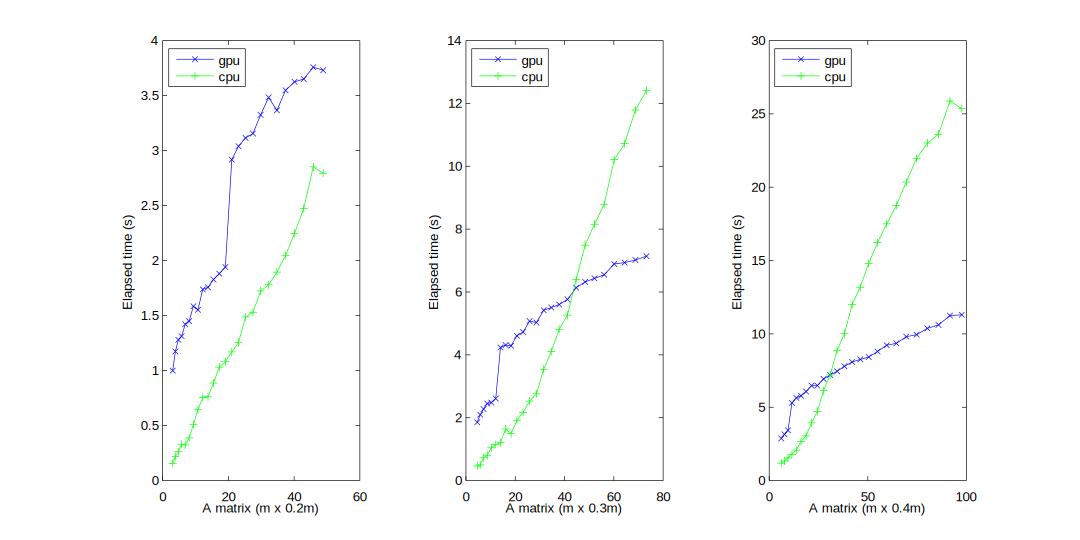
\includegraphics[width=3.5in]{results/random_data/time_vs_matrix_size_constant_tol}
\end{center}
\caption{Speed vs Dimensions of A.  Outer loop tolerance = 0.1.  Inner loop tolerance = $10^{-5}$}
\label{fig:random_data}
\end{figure}

\begin{figure}
\begin{center}
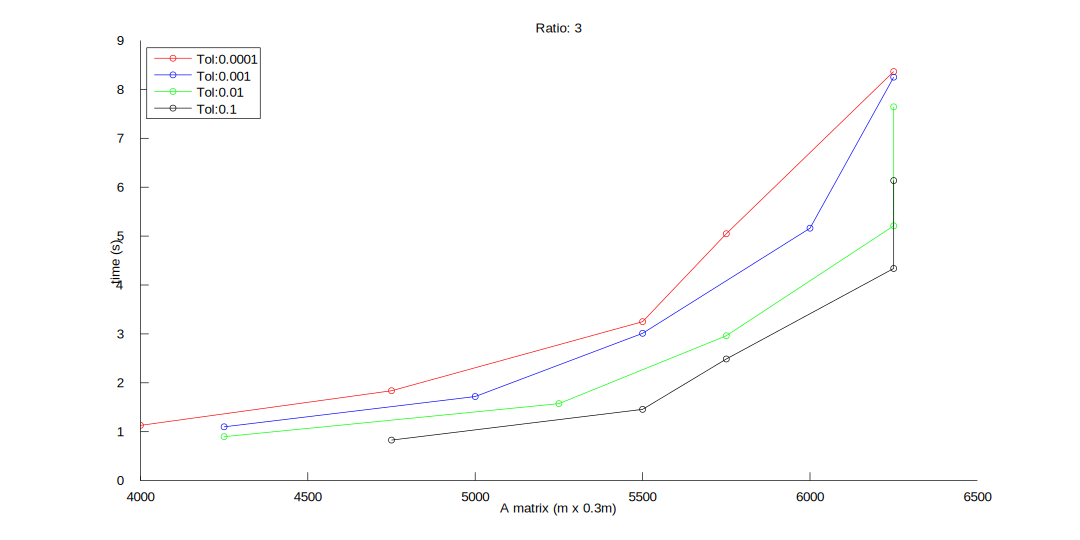
\includegraphics[width=3.5in]{results/random_data/size_vs_speed_crossover_ratio_3}
\end{center}
\caption{Relation between CPU and GPU runtime vs tolerance level}
\label{fig:random_data2}
\end{figure}


\subsection{Face Alignment Stage Benchmark} \label{sec:alignment_benchmark}
This section presents benchmarks of our CPU and GPU implementations of the
alignment stage of the face recognition pipeline described in Algorithm
\ref{alg:iterative_alignment}.  The iterative alignment seeks a similarity
transformation between the coordinate frame of the "camera" resolution test
image and the coordinate frame of the "canonical" resolution images which the
images are compared.  We use a $64$ pixel wide square window in the canonical
frame.  The training images are aligned by manually clicking the two outer eye
corners in the camera frame, and then warping the images via a similarity
transformation such that the eye corners lie at a pair of canonical eye
locations in the canonical frame.  The canonical eye corners are chosen such
that for well aligned images, the canonical window contains exclusively pixels
from the subject's face. 

For experiments on face data we use subsets of the CMU Multi-PIE Face Database.
For gallery images we use frontal images from session 1, which contains 20
images per user taken under different illuminations. For test images we use
images from session 2.  

In Figure \ref{fig:alignment_stage_runtime} we report the time it takes
to align a single test image against each of the users in the gallery.
We vary the size of the gallery to show how implementation scales in the
number of gallery users.
\begin{figure}
\centering
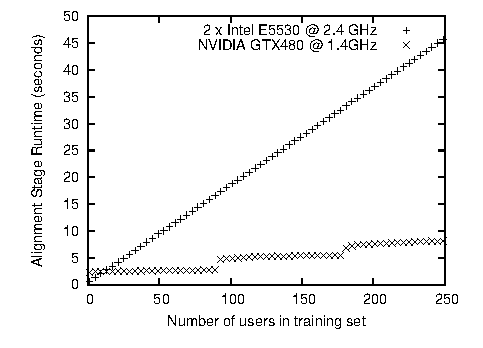
\includegraphics[width=3.4in]{figures/alignment_runtime_graph}
\caption{Alignment Stage Runtime vs. Size of Training Database}
\label{fig:alignment_stage_runtime}
\end{figure}

Previous publications used a hard threshold on the number of subjects kept for the recognition
stage as a compromise between recognition speed and potential recognition rate.
In order to better motivate 
a choice for a threshold of the number of users kept for the recognition stage,
we varied the number of users kept for the recognition stage and estimated the probability
of the test user being among the set of training users kept for the recognition stage.
As can be seen in Figure \ref{fig:user_alignment_rank_plot}, there are rapidly diminishing
returns as the number of kept users is increased beyond ten.  
\begin{figure}
\centering
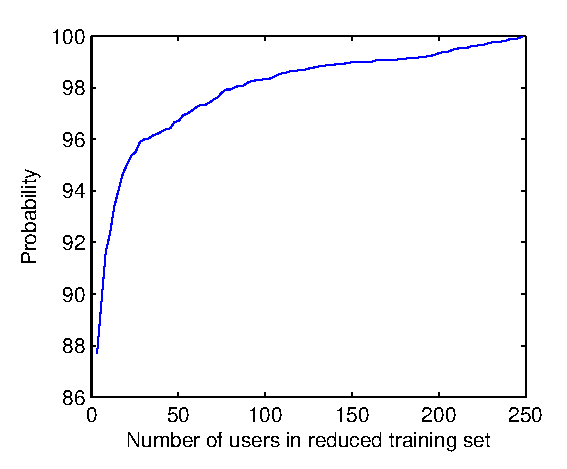
\includegraphics[width=3.4in]{figures/user_alignment_rank_plot}
\caption{Probability of the test user being kept for the recognition stage vs. Number of traning
users kept for the recognition stage}
\label{fig:user_alignment_rank_plot}
\end{figure}

\subsection{Face Recognition Stage Benchmarks}
\label{sec:recognition_benchmark}

\subsection{Face Recognition Pipeline Benchmarks}
\label{sec:pipeline_benchmark}
The fourth experiment compares the recognition rate of the face recognition algorithm at different
image resolutions.  We fixed the number of users to be $enter here$ which was shown in figure  $enter here$  have 95\% probability
to have the true user in the training set, inner loop tolerance to 1e-2 and outer loop tolerance to 1e-3.  

Our final experiment is to compare the speeds of CPU and GPU implementations entire pipeline in Figure \ref{fig:pipeline}.

\section{Conclusion}



\begin{figure}
\centering
\includegraphics[width=3.4in]{figures/alignment_mapping_old}
\caption{Old mapping of alignment parallelism onto cpu concurrency}
\label{fig:alignment_mapping_old}
\end{figure}

\begin{figure}
\centering
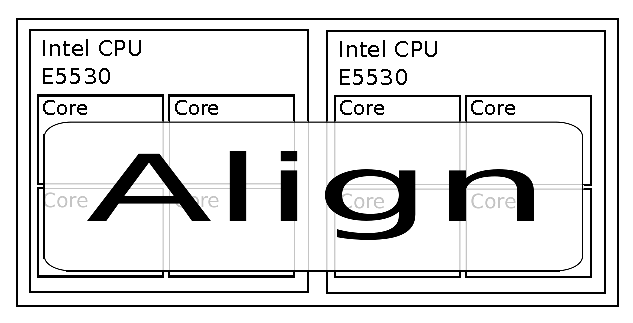
\includegraphics[width=3.4in]{figures/alignment_mapping_cpu}
\caption{Proposed mapping of alignment parallelism onto cpu concurrency}
\label{fig:alignment_mapping_cpu}
\end{figure}

\begin{figure}
\centering
\includegraphics[width=3.4in]{figures/alignment_mapping_gpu}
\caption{Proposed mapping of alignment parallelism onto gpu concurrency}
\label{fig:alignment_mapping_gpu}
\end{figure}

{\small
\bibliographystyle{ieee}
\bibliography{faces}
}

\end{document}
